\PassOptionsToPackage{spanish, es-noshorthands}{babel}
\documentclass[12pt,a4paper]{article}

\usepackage{babel}
\usepackage[utf8]{inputenc}
\usepackage[T1]{fontenc}

\usepackage{amsmath}
\usepackage{amssymb}
\usepackage{amsfonts}
\usepackage{amsthm}

\usepackage{geometry}
\geometry{margin=2.5cm}

\usepackage{tikz}
\usetikzlibrary{arrows.meta, positioning, calc, shapes.geometric}

\usepackage{graphicx}
\usepackage{hyperref}
\usepackage{fancyhdr}
\usepackage{tocloft}
\usepackage{float}
\usepackage{caption}
\usepackage{subcaption}

% Solución definitiva para conflictos de babel con TikZ
\AtBeginDocument{\shorthandoff{"}}

\title{\textbf{\Huge Solucionario Detallado \\ Trabajo Autónomo - Elipse}}

\author{
Basado en la guía de \\ Diego Solís S1, Joaquín Vásquez S2, Benjamín Romo S3 \\
\textit{[Lehmann] Geometría Analítica}
}

\date{INF-112 Cálculo I 2026}

\begin{document}

\maketitle
\thispagestyle{empty}

\vspace{2cm}
\begin{center}
    \Large\textbf{Solucionario Extenso con Explicaciones Paso a Paso}
\end{center}

\newpage
\tableofcontents
\newpage

\section{Introducción a la Elipse}
La elipse es el lugar geométrico de los puntos \(P\) del plano tales que la suma de las distancias a dos puntos fijos (llamados \textbf{focos}) es constante e igual a \(2a\) (longitud del eje mayor).

\textbf{Forma canónica (segunda forma ordinaria):}
\[
\frac{(x-h)^2}{a^2} + \frac{(y-k)^2}{b^2} = 1 \quad (a > b)
\]
o
\[
\frac{(x-h)^2}{b^2} + \frac{(y-k)^2}{a^2} = 1 \quad (a > b)
\]

Relaciones fundamentales:
\[
c^2 = a^2 - b^2, \quad e = \frac{c}{a} \quad (0 < e < 1), \quad \text{Lado recto} = \left| \frac{2b^2}{a} \right|
\]

Centro: \((h,k)\). Vértices y co-vértices según orientación del eje mayor.  
Todas las ecuaciones de esta guía se reducen a esta forma mediante completación de cuadrados.

\newpage
\section{Ejercicios Resueltos}

\subsection{Ejercicio 1}
\textbf{Enunciado:} La ecuación de una elipse es \(x^2 + 4y^2 + 2x - 12y + 6 = 0\). Reducir esta ecuación a la forma ordinaria y determinar las coordenadas del centro, de los vértices y de los focos; calcular las longitudes del eje mayor, del eje menor, de cada lado recto y la excentricidad.

\textbf{Solución paso a paso:}
1. Agrupamos términos:
   \[
   (x^2 + 2x) + 4(y^2 - 3y) + 6 = 0
   \]
2. Completamos cuadrados:
   - Para \(x\): \(x^2 + 2x + 1 = (x+1)^2\)
   - Para \(y\): \(y^2 - 3y + \frac{9}{4} = \left(y - \frac{3}{2}\right)^2\)
3. Sustituimos:
   \[
   (x+1)^2 - 1 + 4\left[\left(y - \frac{3}{2}\right)^2 - \frac{9}{4}\right] + 6 = 0
   \]
   \[
   (x+1)^2 - 1 + 4\left(y - \frac{3}{2}\right)^2 - 9 + 6 = 0
   \]
   \[
   (x+1)^2 + 4\left(y - \frac{3}{2}\right)^2 - 4 = 0
   \]
   \[
   (x+1)^2 + 4\left(y - \frac{3}{2}\right)^2 = 4
   \]
4. Dividimos por 4:
   \[
   \frac{(x+1)^2}{4} + \frac{\left(y - \frac{3}{2}\right)^2}{1} = 1
   \]
5. Forma canónica: eje mayor horizontal (\(a^2 = 4 > b^2 = 1\)).
   - Centro: \((-1, \frac{3}{2})\)
   - \(a = 2\), \(b = 1\)
   - \(c = \sqrt{3}\)
   - Vértices: \((-1 \pm 2, \frac{3}{2})\) → \((1, \frac{3}{2})\) y \((-3, \frac{3}{2})\)
   - Co-vértices: \((-1, \frac{3}{2} \pm 1)\) → \((-1, \frac{5}{2})\) y \((-1, \frac{1}{2})\)
   - Focos: \((-1 \pm \sqrt{3}, \frac{3}{2})\)
   - Longitud eje mayor: \(2a = 4\)
   - Longitud eje menor: \(2b = 2\)
   - Lado recto: \(\frac{2b^2}{a} = 1\)
   - Excentricidad: \(e = \frac{c}{a} = \frac{\sqrt{3}}{2}\)

\textbf{Gráfica:}
\begin{figure}[H]
\centering
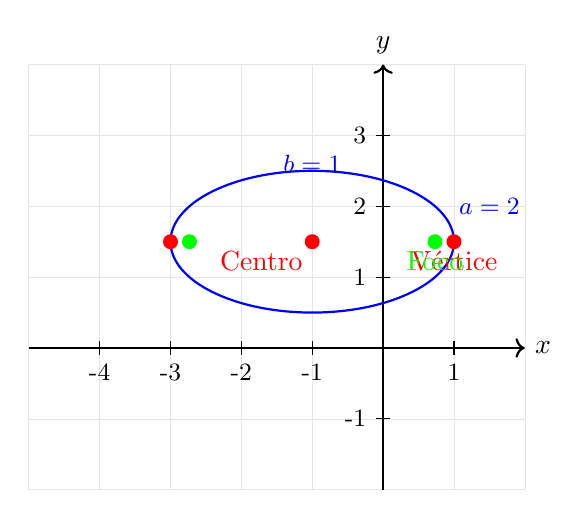
\begin{tikzpicture}[scale=0.9]
    \draw[help lines, color=gray!20] (-5,-2) grid (2,4);
    \draw[thick, ->] (-5,0) -- (2,0) node[right] {$x$};
    \draw[thick, ->] (0,-2) -- (0,4) node[above] {$y$};

    \foreach \x in {-4,-3,-2,-1,1}
        \draw (\x,0.1) -- (\x,-0.1) node[below] {\small \x};
    \foreach \y in {-1,1,2,3}
        \draw (0.1,\y) -- (-0.1,\y) node[left] {\small \y};

    \draw[blue, thick] (-1,1.5) ellipse [x radius=2, y radius=1];
    \fill[red] (-1,1.5) circle (3pt) node[below left] {Centro};
    \fill[red] (1,1.5) circle (3pt) node[below] {Vértice};
    \fill[red] (-3,1.5) circle (3pt);
    \fill[green] (0.732,1.5) circle (3pt) node[below] {Foco};
    \fill[green] (-2.732,1.5) circle (3pt);
    \node[blue] at (1.5,2) {\small \(a=2\)};
    \node[blue] at (-1,2.6) {\small \(b=1\)};
\end{tikzpicture}
\caption{Elipse del Ejercicio 1}
\end{figure}
\newpage

\subsection{Ejercicio 2}
\textbf{Enunciado:} Reducir la ecuación dada a la segunda forma ordinaria de la ecuación de una elipse, y determínense las coordenadas del centro, vértices y focos, las longitudes de los ejes mayor y menor, y la de cada lado recto y la excentricidad:
\[ x^2 + 4y^2 - 6x + 16y + 21 = 0. \]

\textbf{Solución paso a paso:}
1. Agrupamos:
   \[
   (x^2 - 6x) + 4(y^2 + 4y) + 21 = 0
   \]
2. Completamos cuadrados:
   - \(x^2 - 6x + 9 = (x-3)^2\)
   - \(y^2 + 4y + 4 = (y+2)^2\)
3. Sustituimos:
   \[
   (x-3)^2 - 9 + 4[(y+2)^2 - 4] + 21 = 0
   \]
   \[
   (x-3)^2 - 9 + 4(y+2)^2 - 16 + 21 = 0
   \]
   \[
   (x-3)^2 + 4(y+2)^2 - 4 = 0
   \]
   \[
   (x-3)^2 + 4(y+2)^2 = 4
   \]
4. Dividimos por 4:
   \[
   \frac{(x-3)^2}{4} + (y+2)^2 = 1
   \]
5. Eje mayor horizontal (\(a^2=4 > b^2=1\)):
   - Centro: \((3, -2)\)
   - \(a=2\), \(b=1\)
   - \(c=\sqrt{3}\)
   - Vértices: \((3\pm2, -2)\)
   - Co-vértices: \((3, -2\pm1)\)
   - Focos: \((3\pm\sqrt{3}, -2)\)
   - Eje mayor: 4; eje menor: 2
   - Lado recto: 1
   - \(e = \frac{\sqrt{3}}{2}\)

\textbf{Gráfica:}
\begin{figure}[H]
\centering
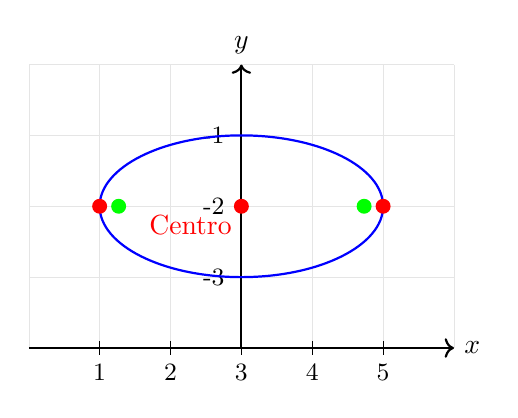
\begin{tikzpicture}[scale=0.9]
    \draw[help lines, color=gray!20] (0,-4) grid (6,0);
    \draw[thick, ->] (0,-4) -- (6,-4) node[right] {$x$};
    \draw[thick, ->] (3,-4) -- (3,0) node[above] {$y$};

    \foreach \x in {1,2,3,4,5}
        \draw (\x,-3.9) -- (\x,-4.1) node[below] {\small \x};
    \foreach \y in {-3,-2,-1}
        \draw (3.1,\y) -- (2.9,\y) node[left] {\small \y};

    \draw[blue, thick] (3,-2) ellipse [x radius=2, y radius=1];
    \fill[red] (3,-2) circle (3pt) node[below left] {Centro};
    \fill[red] (5,-2) circle (3pt);
    \fill[red] (1,-2) circle (3pt);
    \fill[green] (4.732,-2) circle (3pt);
    \fill[green] (1.268,-2) circle (3pt);
\end{tikzpicture}
\caption{Elipse del Ejercicio 2}
\end{figure}
\newpage

\subsection{Ejercicio 3}
\textbf{Enunciado:} \(4x^2 + 9y^2 + 32x - 18y + 37 = 0\).

\textbf{Solución paso a paso:}
1. Agrupamos:
   \[
   4(x^2 + 8x) + 9(y^2 - 2y) + 37 = 0
   \]
2. Completamos:
   - \(x^2 + 8x + 16 = (x+4)^2\)
   - \(y^2 - 2y + 1 = (y-1)^2\)
3. Sustituimos y simplificamos:
   \[
   4[(x+4)^2 - 16] + 9[(y-1)^2 - 1] + 37 = 0
   \]
   \[
   4(x+4)^2 - 64 + 9(y-1)^2 - 9 + 37 = 0
   \]
   \[
   4(x+4)^2 + 9(y-1)^2 = 36
   \]
4. Dividimos por 36:
   \[
   \frac{(x+4)^2}{9} + \frac{(y-1)^2}{4} = 1
   \]
5. Eje mayor horizontal (\(a=3\), \(b=2\)):
   - Centro: \((-4, 1)\)
   - \(c = \sqrt{5}\)
   - Vértices: \((-4 \pm 3, 1)\)
   - Co-vértices: \((-4, 1 \pm 2)\)
   - Focos: \((-4 \pm \sqrt{5}, 1)\)
   - Eje mayor: 6; eje menor: 4
   - Lado recto: \(\frac{8}{3}\)
   - \(e = \frac{\sqrt{5}}{3}\)

\textbf{Gráfica:}
\begin{figure}[H]
\centering
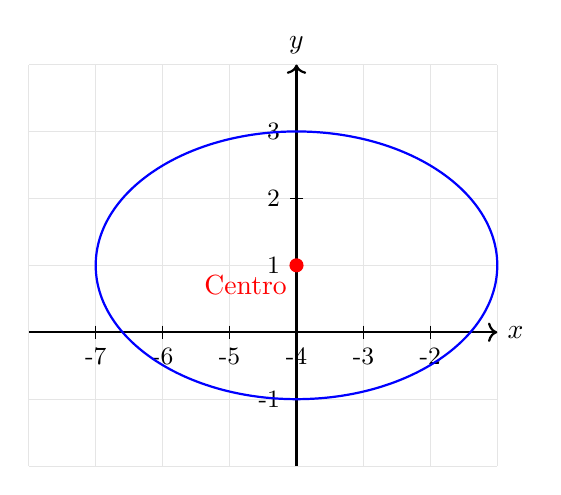
\begin{tikzpicture}[scale=0.85]
    \draw[help lines, color=gray!20] (-8,-2) grid (-1,4);
    \draw[thick, ->] (-8,0) -- (-1,0) node[right] {$x$};
    \draw[thick, ->] (-4,-2) -- (-4,4) node[above] {$y$};

    \foreach \x in {-7,-6,-5,-4,-3,-2}
        \draw (\x,0.1) -- (\x,-0.1) node[below] {\small \x};
    \foreach \y in {-1,1,2,3}
        \draw (-3.9,\y) -- (-4.1,\y) node[left] {\small \y};

    \draw[blue, thick] (-4,1) ellipse [x radius=3, y radius=2];
    \fill[red] (-4,1) circle (3pt) node[below left] {Centro};
\end{tikzpicture}
\caption{Elipse del Ejercicio 3}
\end{figure}
\newpage

\subsection{Ejercicio 4}
\textbf{Enunciado:} \(x^2 + 4y^2 - 10x - 40y + 109 = 0\).

\textbf{Solución paso a paso:}
1. Agrupamos y completamos:
   \[
   (x^2 - 10x) + 4(y^2 - 10y) + 109 = 0
   \]
   \[
   (x-5)^2 - 25 + 4[(y-5)^2 - 25] + 109 = 0
   \]
   \[
   (x-5)^2 + 4(y-5)^2 - 16 = 0
   \]
   \[
   (x-5)^2 + 4(y-5)^2 = 16
   \]
2. Dividimos por 16:
   \[
   \frac{(x-5)^2}{16} + \frac{(y-5)^2}{4} = 1
   \]
3. Eje mayor horizontal (\(a=4\), \(b=2\)):
   - Centro: \((5, 5)\)
   - \(c = 2\sqrt{3}\)
   - Vértices: \((5 \pm 4, 5)\)
   - Focos: \((5 \pm 2\sqrt{3}, 5)\)
   - Eje mayor: 8; eje menor: 4
   - Lado recto: 2
   - \(e = \frac{\sqrt{3}}{2}\)

\textbf{Gráfica:}
\begin{figure}[H]
\centering
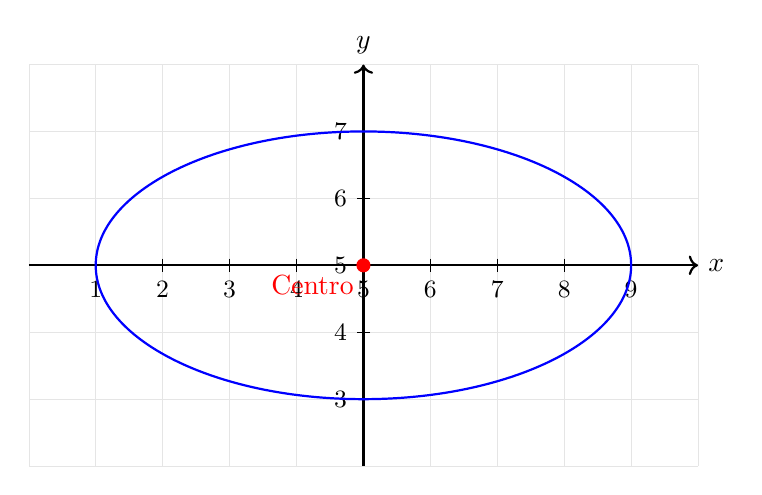
\begin{tikzpicture}[scale=0.85]
    \draw[help lines, color=gray!20] (0,2) grid (10,8);
    \draw[thick, ->] (0,5) -- (10,5) node[right] {$x$};
    \draw[thick, ->] (5,2) -- (5,8) node[above] {$y$};

    \foreach \x in {1,2,3,4,5,6,7,8,9}
        \draw (\x,5.1) -- (\x,4.9) node[below] {\small \x};
    \foreach \y in {3,4,5,6,7}
        \draw (5.1,\y) -- (4.9,\y) node[left] {\small \y};

    \draw[blue, thick] (5,5) ellipse [x radius=4, y radius=2];
    \fill[red] (5,5) circle (3pt) node[below left] {Centro};
\end{tikzpicture}
\caption{Elipse del Ejercicio 4}
\end{figure}
\newpage

\subsection{Ejercicio 5}
\textbf{Enunciado:} \(9x^2 + 4y^2 - 8y - 32 = 0\).

\textbf{Solución paso a paso:}
1. Agrupamos:
   \[
   9x^2 + 4(y^2 - 2y) - 32 = 0
   \]
2. Completamos el cuadrado en \(y\):
   \[
   9x^2 + 4[(y-1)^2 - 1] - 32 = 0
   \]
   \[
   9x^2 + 4(y-1)^2 = 36
   \]
3. Dividimos por 36:
   \[
   \frac{x^2}{4} + \frac{(y-1)^2}{9} = 1
   \]
4. Eje mayor vertical (\(a=3\), \(b=2\)):
   - Centro: \((0, 1)\)
   - \(c = \sqrt{5}\)
   - Vértices: \((0, 1 \pm 3)\)
   - Focos: \((0, 1 \pm \sqrt{5})\)
   - Eje mayor: 6; eje menor: 4
   - Lado recto: \(\frac{8}{3}\)
   - \(e = \frac{\sqrt{5}}{3}\)

\textbf{Gráfica:}
\begin{figure}[H]
\centering
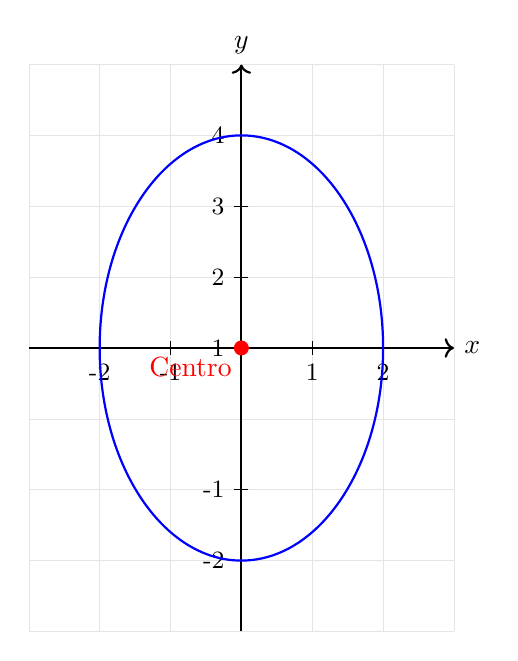
\begin{tikzpicture}[scale=0.9]
    \draw[help lines, color=gray!20] (-3,-3) grid (3,5);
    \draw[thick, ->] (-3,1) -- (3,1) node[right] {$x$};
    \draw[thick, ->] (0,-3) -- (0,5) node[above] {$y$};

    \foreach \x in {-2,-1,1,2}
        \draw (\x,1.1) -- (\x,0.9) node[below] {\small \x};
    \foreach \y in {-2,-1,1,2,3,4}
        \draw (0.1,\y) -- (-0.1,\y) node[left] {\small \y};

    \draw[blue, thick] (0,1) ellipse [x radius=2, y radius=3];
    \fill[red] (0,1) circle (3pt) node[below left] {Centro};
\end{tikzpicture}
\caption{Elipse del Ejercicio 5}
\end{figure}
\newpage

\subsection{Ejercicio 6}
\textbf{Enunciado:} Hallar la ecuación de la elipse cuyos vértices son los puntos \((4,0)\), \((-4,0)\), y cuyos focos son los puntos \((3,0)\), \((-3,0)\).

\textbf{Solución paso a paso:}
1. Vértices en \((\pm 4, 0)\) → centro \((0,0)\), eje mayor horizontal, \(a=4\).
2. Focos en \((\pm 3, 0)\) → \(c=3\).
3. \(b^2 = a^2 - c^2 = 16 - 9 = 7\).
4. Ecuación:
   \[
   \frac{x^2}{16} + \frac{y^2}{7} = 1
   \]

\textbf{Gráfica:}
\begin{figure}[H]
\centering
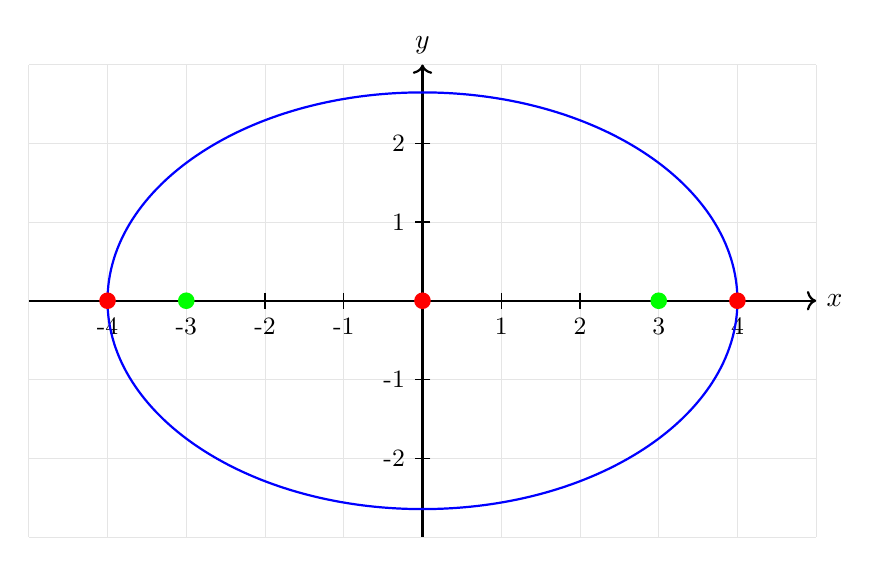
\begin{tikzpicture}[scale=1]
    \draw[help lines, color=gray!20] (-5,-3) grid (5,3);
    \draw[thick, ->] (-5,0) -- (5,0) node[right] {$x$};
    \draw[thick, ->] (0,-3) -- (0,3) node[above] {$y$};

    \foreach \x in {-4,-3,-2,-1,1,2,3,4}
        \draw (\x,0.1) -- (\x,-0.1) node[below] {\small \x};
    \foreach \y in {-2,-1,1,2}
        \draw (0.1,\y) -- (-0.1,\y) node[left] {\small \y};

    \draw[blue, thick] (0,0) ellipse [x radius=4, y radius=2.646];
    \fill[red] (0,0) circle (3pt);
    \fill[red] (4,0) circle (3pt);
    \fill[red] (-4,0) circle (3pt);
    \fill[green] (3,0) circle (3pt);
    \fill[green] (-3,0) circle (3pt);
\end{tikzpicture}
\caption{Elipse del Ejercicio 6}
\end{figure}
\newpage

\subsection{Ejercicio 7}
\textbf{Enunciado:} Los vértices de una elipse son los puntos \((0,6)\), \((0,-6)\), y sus focos son los puntos \((0,4)\), \((0,-4)\). Hallar su ecuación.

\textbf{Solución paso a paso:}
1. Vértices en \((0, \pm 6)\) → centro \((0,0)\), eje mayor vertical, \(a=6\).
2. Focos en \((0, \pm 4)\) → \(c=4\).
3. \(b^2 = a^2 - c^2 = 36 - 16 = 20\).
4. Ecuación:
   \[
   \frac{x^2}{20} + \frac{y^2}{36} = 1
   \]

\textbf{Gráfica:}
\begin{figure}[H]
\centering
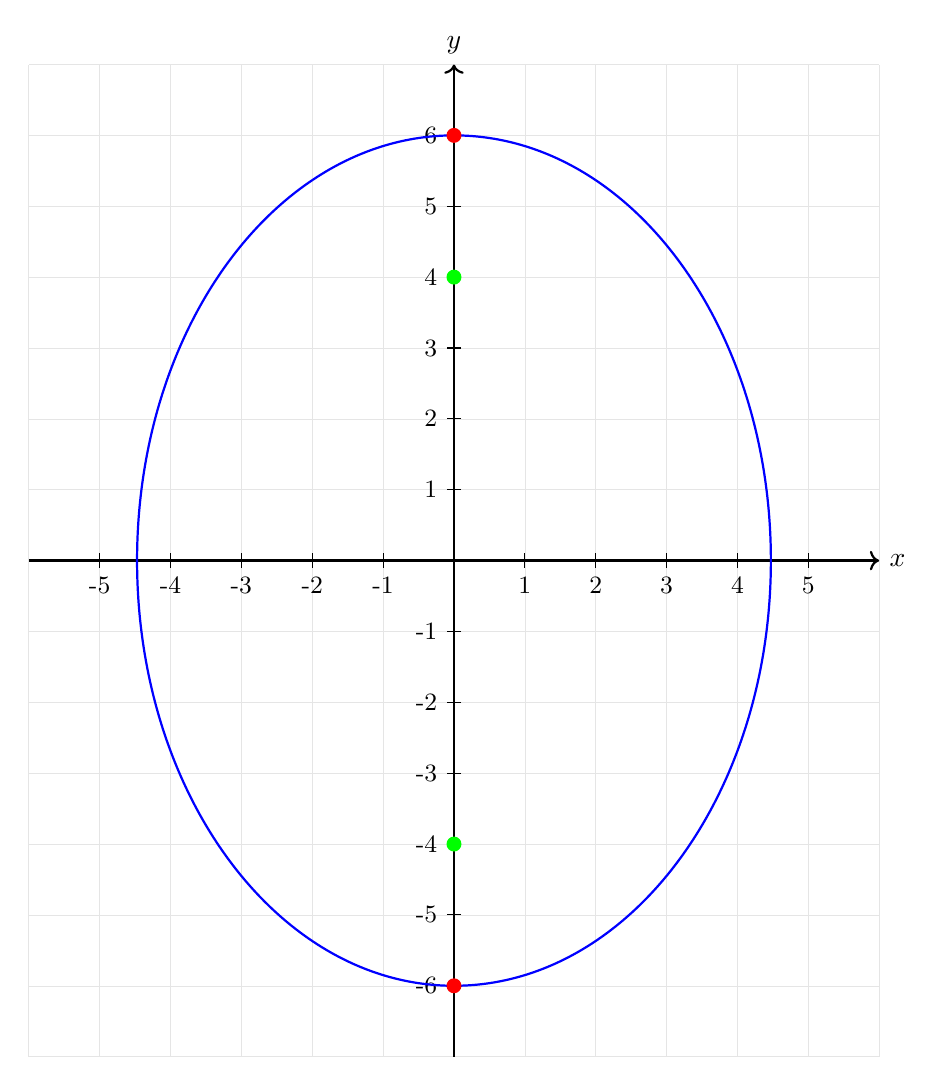
\begin{tikzpicture}[scale=0.9]
    \draw[help lines, color=gray!20] (-6,-7) grid (6,7);
    \draw[thick, ->] (-6,0) -- (6,0) node[right] {$x$};
    \draw[thick, ->] (0,-7) -- (0,7) node[above] {$y$};

    \foreach \x in {-5,-4,-3,-2,-1,1,2,3,4,5}
        \draw (\x,0.1) -- (\x,-0.1) node[below] {\small \x};
    \foreach \y in {-6,-5,-4,-3,-2,-1,1,2,3,4,5,6}
        \draw (0.1,\y) -- (-0.1,\y) node[left] {\small \y};

    \draw[blue, thick] (0,0) ellipse [x radius=4.472, y radius=6];
    \fill[red] (0,6) circle (3pt);
    \fill[red] (0,-6) circle (3pt);
    \fill[green] (0,4) circle (3pt);
    \fill[green] (0,-4) circle (3pt);
\end{tikzpicture}
\caption{Elipse del Ejercicio 7}
\end{figure}
\newpage

\subsection{Ejercicio 8}
\textbf{Enunciado:} Hallar la ecuación de la elipse cuyos focos son los puntos \((2,0)\), \((-2,0)\), y su excentricidad es igual a \(\frac{2}{3}\).

\textbf{Solución paso a paso:}
1. Focos \((\pm 2,0)\) → centro \((0,0)\), eje mayor horizontal, \(c=2\).
2. \(e = \frac{c}{a} = \frac{2}{3}\) → \(a = 3\).
3. \(b^2 = a^2 - c^2 = 9 - 4 = 5\).
4. Ecuación:
   \[
   \frac{x^2}{9} + \frac{y^2}{5} = 1
   \]

\textbf{Gráfica:}
\begin{figure}[H]
\centering
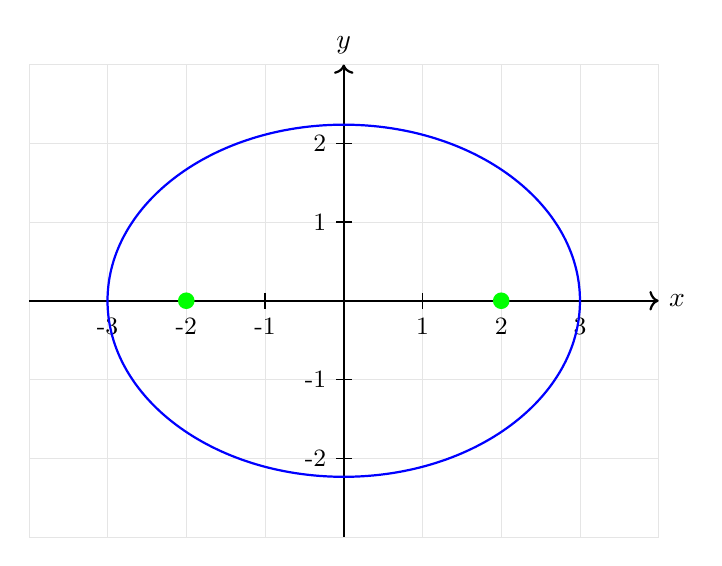
\begin{tikzpicture}[scale=1]
    \draw[help lines, color=gray!20] (-4,-3) grid (4,3);
    \draw[thick, ->] (-4,0) -- (4,0) node[right] {$x$};
    \draw[thick, ->] (0,-3) -- (0,3) node[above] {$y$};

    \foreach \x in {-3,-2,-1,1,2,3}
        \draw (\x,0.1) -- (\x,-0.1) node[below] {\small \x};
    \foreach \y in {-2,-1,1,2}
        \draw (0.1,\y) -- (-0.1,\y) node[left] {\small \y};

    \draw[blue, thick] (0,0) ellipse [x radius=3, y radius=2.236];
    \fill[green] (2,0) circle (3pt);
    \fill[green] (-2,0) circle (3pt);
\end{tikzpicture}
\caption{Elipse del Ejercicio 8}
\end{figure}
\newpage

\subsection{Ejercicio 9}
\textbf{Enunciado:} Los focos de una elipse son los puntos \((3,0)\), \((-3,0)\), y la longitud de uno cualquiera de sus lados rectos es igual a 9. Hallar la ecuación de la elipse.

\textbf{Solución paso a paso:}
1. \(c=3\), lado recto \(\frac{2b^2}{a} = 9\).
2. \(b^2 = \frac{9a}{2}\).
3. \(c^2 = a^2 - b^2\) → \(9 = a^2 - \frac{9a}{2}\).
4. \(2a^2 - 9a - 18 = 0\) → \(a = 6\) (raíz positiva).
5. \(b^2 = 27\).
6. Ecuación:
   \[
   \frac{x^2}{36} + \frac{y^2}{27} = 1
   \]

\textbf{Gráfica:}
\begin{figure}[H]
\centering
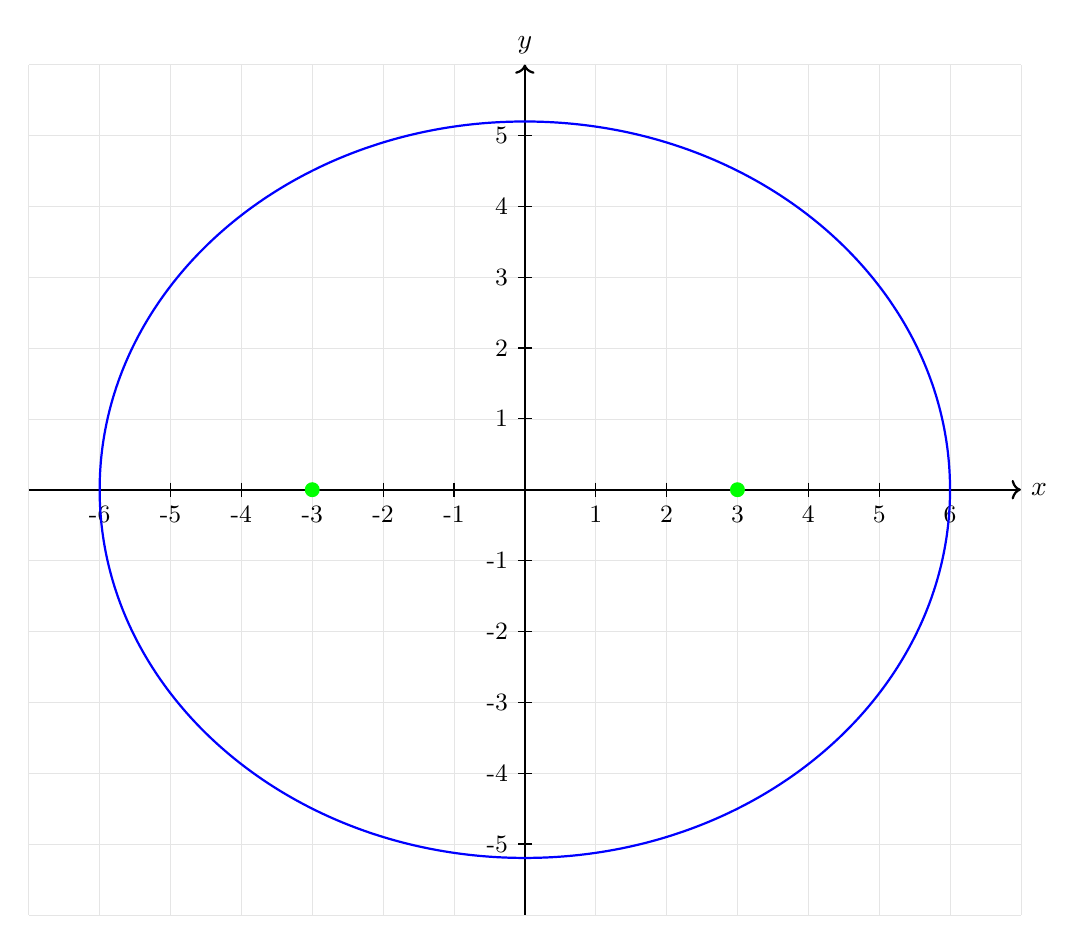
\begin{tikzpicture}[scale=0.9]
    \draw[help lines, color=gray!20] (-7,-6) grid (7,6);
    \draw[thick, ->] (-7,0) -- (7,0) node[right] {$x$};
    \draw[thick, ->] (0,-6) -- (0,6) node[above] {$y$};

    \foreach \x in {-6,-5,-4,-3,-2,-1,1,2,3,4,5,6}
        \draw (\x,0.1) -- (\x,-0.1) node[below] {\small \x};
    \foreach \y in {-5,-4,-3,-2,-1,1,2,3,4,5}
        \draw (0.1,\y) -- (-0.1,\y) node[left] {\small \y};

    \draw[blue, thick] (0,0) ellipse [x radius=6, y radius=5.196];
    \fill[green] (3,0) circle (3pt);
    \fill[green] (-3,0) circle (3pt);
\end{tikzpicture}
\caption{Elipse del Ejercicio 9}
\end{figure}
\newpage

\subsection{Ejercicio 10}
\textbf{Enunciado:} Hallar la ecuación y la excentricidad de la elipse que tiene su centro en el origen, uno de sus vértices en el punto \((0, -7)\) y pasa por el punto \(\left(\sqrt{5}, \frac{14}{3}\right)\).

\textbf{Solución paso a paso:}
1. Vértice \((0,-7)\) → eje mayor vertical, \(a=7\), centro \((0,0)\).
2. Ecuación: \(\frac{x^2}{b^2} + \frac{y^2}{49} = 1\).
3. Sustituimos punto:
   \[
   \frac{5}{b^2} + \frac{(196/9)}{49} = 1 \implies \frac{5}{b^2} + \frac{4}{9} = 1 \implies b^2 = 9
   \]
4. Ecuación: \(\frac{x^2}{9} + \frac{y^2}{49} = 1\).
5. \(c = \sqrt{40} = 2\sqrt{10}\), \(e = \frac{2\sqrt{10}}{7}\).

\textbf{Gráfica:}
\begin{figure}[H]
\centering
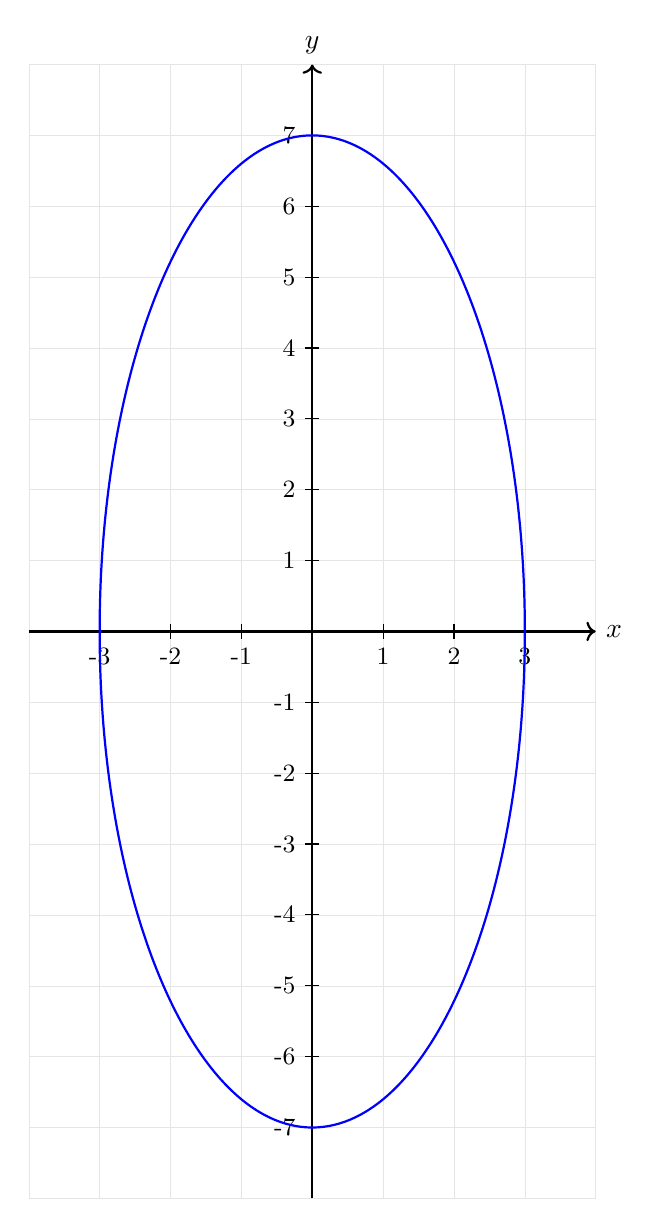
\begin{tikzpicture}[scale=0.9]
    \draw[help lines, color=gray!20] (-4,-8) grid (4,8);
    \draw[thick, ->] (-4,0) -- (4,0) node[right] {$x$};
    \draw[thick, ->] (0,-8) -- (0,8) node[above] {$y$};

    \foreach \x in {-3,-2,-1,1,2,3}
        \draw (\x,0.1) -- (\x,-0.1) node[below] {\small \x};
    \foreach \y in {-7,-6,-5,-4,-3,-2,-1,1,2,3,4,5,6,7}
        \draw (0.1,\y) -- (-0.1,\y) node[left] {\small \y};

    \draw[blue, thick] (0,0) ellipse [x radius=3, y radius=7];
\end{tikzpicture}
\caption{Elipse del Ejercicio 10}
\end{figure}
\newpage

\subsection{Ejercicio 11}
\textbf{Enunciado:} Una elipse tiene su centro en el origen y su eje mayor coincide con el eje X. Hallar su ecuación sabiendo que pasa por los puntos \((\sqrt{6}, -1)\) y \((2, \sqrt{2})\).

\textbf{Solución paso a paso:}
1. Eje mayor horizontal: \(\frac{x^2}{a^2} + \frac{y^2}{b^2} = 1\).
2. Sistema:
   \[
   \frac{6}{a^2} + \frac{1}{b^2} = 1, \quad \frac{4}{a^2} + \frac{2}{b^2} = 1
   \]
3. Resolución: \(a^2 = 8\), \(b^2 = 4\).
4. Ecuación: \(\frac{x^2}{8} + \frac{y^2}{4} = 1\).

\textbf{Gráfica:}
\begin{figure}[H]
\centering
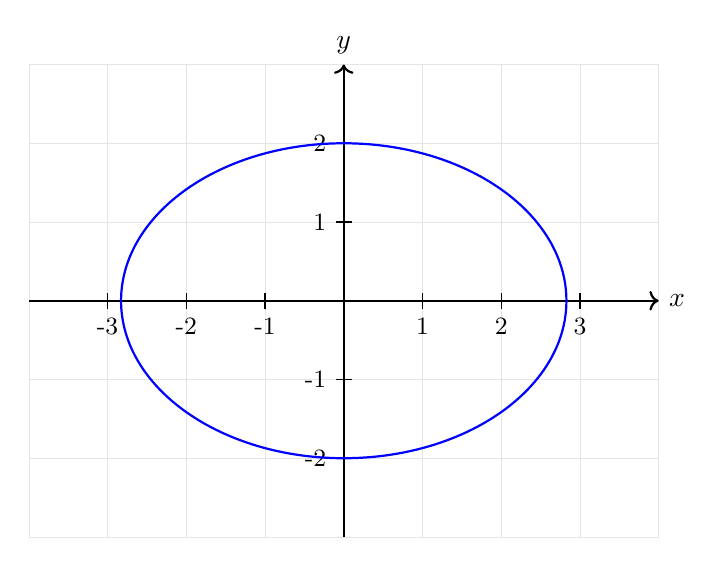
\begin{tikzpicture}[scale=1]
    \draw[help lines, color=gray!20] (-4,-3) grid (4,3);
    \draw[thick, ->] (-4,0) -- (4,0) node[right] {$x$};
    \draw[thick, ->] (0,-3) -- (0,3) node[above] {$y$};

    \foreach \x in {-3,-2,-1,1,2,3}
        \draw (\x,0.1) -- (\x,-0.1) node[below] {\small \x};
    \foreach \y in {-2,-1,1,2}
        \draw (0.1,\y) -- (-0.1,\y) node[left] {\small \y};

    \draw[blue, thick] (0,0) ellipse [x radius=2.828, y radius=2];
\end{tikzpicture}
\caption{Elipse del Ejercicio 11}
\end{figure}
\newpage

\subsection{Ejercicio 12}
\textbf{Enunciado:} Focos \((3,8)\) y \((3,2)\); longitud del eje mayor \(= 10\).

\textbf{Solución paso a paso:}
1. Centro: \((3,5)\), \(2c = 6\) → \(c=3\), eje mayor vertical (\(2a=10\) → \(a=5\)).
2. \(b^2 = 25 - 9 = 16\).
3. Ecuación:
   \[
   \frac{(x-3)^2}{16} + \frac{(y-5)^2}{25} = 1
   \]

\textbf{Gráfica:}
\begin{figure}[H]
\centering
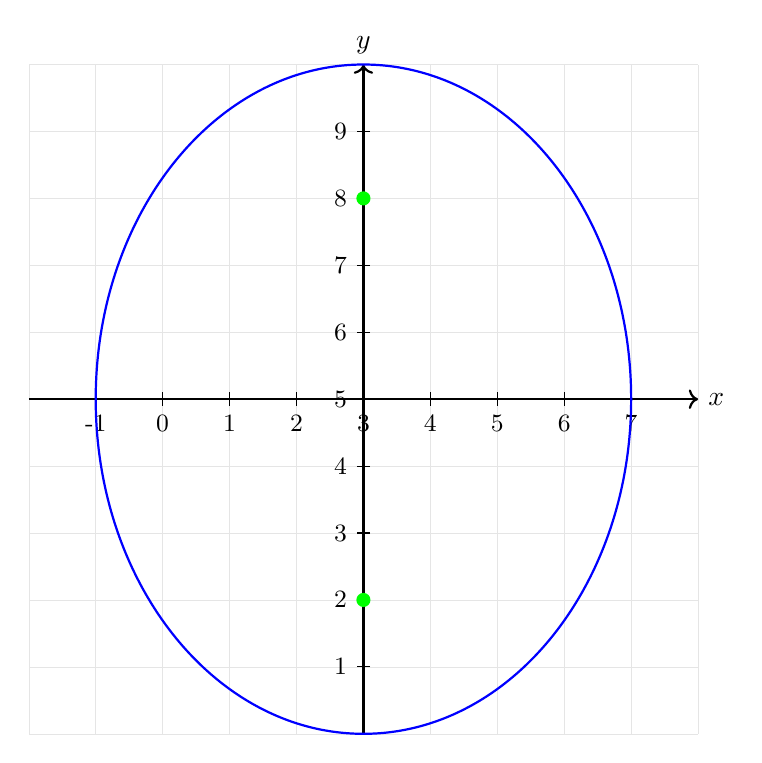
\begin{tikzpicture}[scale=0.85]
    \draw[help lines, color=gray!20] (-2,0) grid (8,10);
    \draw[thick, ->] (-2,5) -- (8,5) node[right] {$x$};
    \draw[thick, ->] (3,0) -- (3,10) node[above] {$y$};

    \foreach \x in {-1,0,1,2,3,4,5,6,7}
        \draw (\x,5.1) -- (\x,4.9) node[below] {\small \x};
    \foreach \y in {1,2,3,4,5,6,7,8,9}
        \draw (3.1,\y) -- (2.9,\y) node[left] {\small \y};

    \draw[blue, thick] (3,5) ellipse [x radius=4, y radius=5];
    \fill[green] (3,8) circle (3pt);
    \fill[green] (3,2) circle (3pt);
\end{tikzpicture}
\caption{Elipse del Ejercicio 12}
\end{figure}
\newpage

\subsection{Ejercicio 13}
\textbf{Enunciado:} Vértices \((-3,-1)\) y \((5,-1)\); excentricidad \(= \frac{3}{4}\).

\textbf{Solución paso a paso:}
1. Centro: \((1,-1)\), \(a=4\) (horizontal).
2. \(c = \frac{3}{4} \cdot 4 = 3\).
3. \(b^2 = 16 - 9 = 7\).
4. Ecuación:
   \[
   \frac{(x-1)^2}{16} + \frac{(y+1)^2}{7} = 1
   \]

\textbf{Gráfica:}
\begin{figure}[H]
\centering
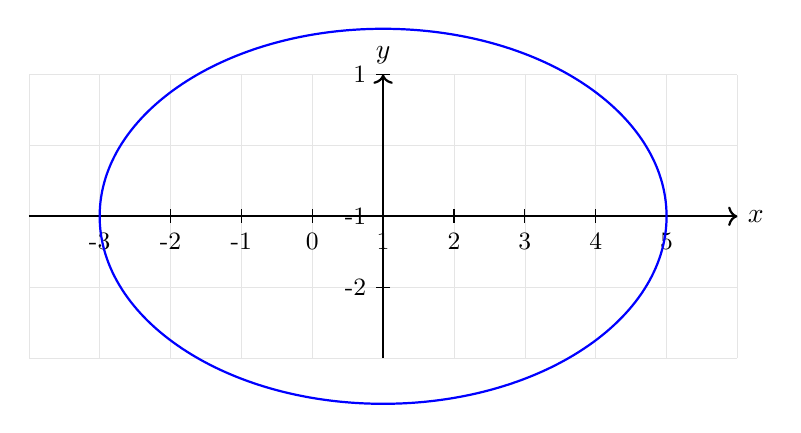
\begin{tikzpicture}[scale=0.9]
    \draw[help lines, color=gray!20] (-4,-3) grid (6,1);
    \draw[thick, ->] (-4,-1) -- (6,-1) node[right] {$x$};
    \draw[thick, ->] (1,-3) -- (1,1) node[above] {$y$};

    \foreach \x in {-3,-2,-1,0,1,2,3,4,5}
        \draw (\x,-0.9) -- (\x,-1.1) node[below] {\small \x};
    \foreach \y in {-2,-1,1}
        \draw (1.1,\y) -- (0.9,\y) node[left] {\small \y};

    \draw[blue, thick] (1,-1) ellipse [x radius=4, y radius=2.646];
\end{tikzpicture}
\caption{Elipse del Ejercicio 13}
\end{figure}
\newpage

\subsection{Ejercicio 14}
\textbf{Enunciado:} Vértices \((2,6)\) y \((2,-2)\); longitud del lado recto \(= 2\).

\textbf{Solución paso a paso:}
1. Centro: \((2,2)\), eje mayor vertical, \(a=4\).
2. Lado recto \(\frac{2b^2}{a} = 2\) → \(b^2 = 4\).
3. Ecuación:
   \[
   \frac{(x-2)^2}{4} + \frac{(y-2)^2}{16} = 1
   \]

\textbf{Gráfica:}
\begin{figure}[H]
\centering
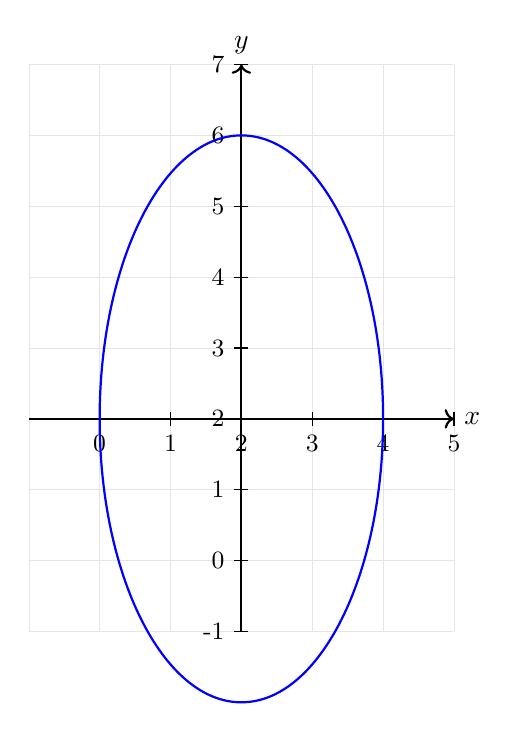
\begin{tikzpicture}[scale=0.9]
    \draw[help lines, color=gray!20] (-1,-1) grid (5,7);
    \draw[thick, ->] (-1,2) -- (5,2) node[right] {$x$};
    \draw[thick, ->] (2,-1) -- (2,7) node[above] {$y$};

    \foreach \x in {0,1,2,3,4,5}
        \draw (\x,2.1) -- (\x,1.9) node[below] {\small \x};
    \foreach \y in {-1,0,1,2,3,4,5,6,7}
        \draw (2.1,\y) -- (1.9,\y) node[left] {\small \y};

    \draw[blue, thick] (2,2) ellipse [x radius=2, y radius=4];
\end{tikzpicture}
\caption{Elipse del Ejercicio 14}
\end{figure}
\newpage

\subsection{Ejercicio 15}
\textbf{Enunciado:} La ecuación de una familia de elipses es \(kx^2 + 4y^2 + 6x - 8y - 5 = 0\). Hallar las ecuaciones de aquellos elementos de la familia que tienen una excentricidad igual a \(\frac{1}{2}\).

\textbf{Solución paso a paso corregida:}

1. Completamos cuadrados (para \(k \neq 0\)):
   \[
   k\left(x^2 + \frac{6}{k}x\right) + 4(y^2 - 2y) - 5 = 0
   \]
   \[
   k\left[\left(x + \frac{3}{k}\right)^2 - \frac{9}{k^2}\right] + 4\bigl[(y-1)^2 - 1\bigr] - 5 = 0
   \]
   \[
   k\left(x + \frac{3}{k}\right)^2 - \frac{9}{k} + 4(y-1)^2 - 4 - 5 = 0
   \]
   \[
   k\left(x + \frac{3}{k}\right)^2 + 4(y-1)^2 = 9 + \frac{9}{k}
   \]
   \[
   \frac{\left(x + \frac{3}{k}\right)^2}{\frac{9(1+k)}{k^2}} + \frac{(y-1)^2}{\frac{9(1+k)}{4k}} = 1
   \]

2. Para que represente una elipse, ambos denominadores deben ser positivos. Tomamos \(k>0\).

   - **Eje mayor horizontal** si \(\displaystyle \frac{9(1+k)}{k^2} > \frac{9(1+k)}{4k}\), lo que ocurre para \(0<k<4\).  
     En este caso, \(a^2 = \frac{9(1+k)}{k^2}\), \(b^2 = \frac{9(1+k)}{4k}\).  
     La condición \(e = \frac{1}{2}\) implica \(b^2 = \frac{3}{4}a^2\):
     \[
     \frac{9(1+k)}{4k} = \frac{3}{4}\cdot\frac{9(1+k)}{k^2} \;\Longrightarrow\; \frac{1}{4k} = \frac{3}{4k^2} \;\Longrightarrow\; k = 3.
     \]
   - **Eje mayor vertical** si \(k>4\). Ahora \(a^2 = \frac{9(1+k)}{4k}\), \(b^2 = \frac{9(1+k)}{k^2}\).  
     De \(b^2 = \frac{3}{4}a^2\):
     \[
     \frac{9(1+k)}{k^2} = \frac{3}{4}\cdot\frac{9(1+k)}{4k} \;\Longrightarrow\; \frac{1}{k^2} = \frac{3}{16k} \;\Longrightarrow\; k = \frac{16}{3}.
     \]

3. Sustituyendo estos valores:

   - Para \(k = 3\):
     \[
     \frac{(x+1)^2}{4} + \frac{(y-1)^2}{3} = 1.
     \]
   - Para \(k = \frac{16}{3}\):
     \[
     \frac{(x+9/16)^2}{513/256} + \frac{(y-1)^2}{171/64} = 1,
     \]
     o bien, con enteros,
     \[
     \frac{256(x+9/16)^2}{513} + \frac{64(y-1)^2}{171} = 1.
     \]

\textbf{Gráfica de ambas:}
\begin{figure}[H]
\centering
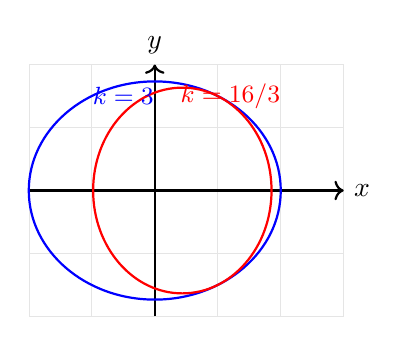
\begin{tikzpicture}[scale=0.8]
    \draw[help lines, color=gray!20] (-3,-1) grid (2,3);
    \draw[thick, ->] (-3,1) -- (2,1) node[right] {$x$};
    \draw[thick, ->] (-1,-1) -- (-1,3) node[above] {$y$};

    % Elipse con k=3: centro (-1,1), a=2, b≈1.732
    \draw[blue, thick] (-1,1) ellipse [x radius=2, y radius=1.732];
    % Elipse con k=16/3: centro (-0.5625,1), a≈1.633, b≈1.416
    \draw[red, thick] (-0.5625,1) ellipse [x radius=1.416, y radius=1.633];
    \node[blue] at (-1.5,2.5) {\small \(k=3\)};
    \node[red] at (0.2,2.5) {\small \(k=16/3\)};
\end{tikzpicture}
\caption{Familia con \(e=1/2\)}
\end{figure}
\newpage

\subsection{Ejercicio 16}
\textbf{Enunciado:} Hallar las longitudes de los radios vectores del punto \((2,1)\) de la elipse \(9x^2 + y^2 -18x -2y + 1 = 0\).

\textbf{Solución paso a paso:}
1. Reducción:
   \[
   9(x-1)^2 + (y-1)^2 = 9 \implies \frac{(x-1)^2}{1} + \frac{(y-1)^2}{9} = 1
   \]
   (eje mayor vertical, \(a=3\), \(b=1\), centro \((1,1)\), \(c=2\sqrt{2}\)).
2. Focos: \((1, 1 \pm 2\sqrt{2})\).
3. Punto \((2,1)\) (extremo del eje menor).
4. Distancia a cada foco: ambas igual a 3 (por propiedad: suma = \(2a = 6\)).

\textbf{Gráfica:}
\begin{figure}[H]
\centering
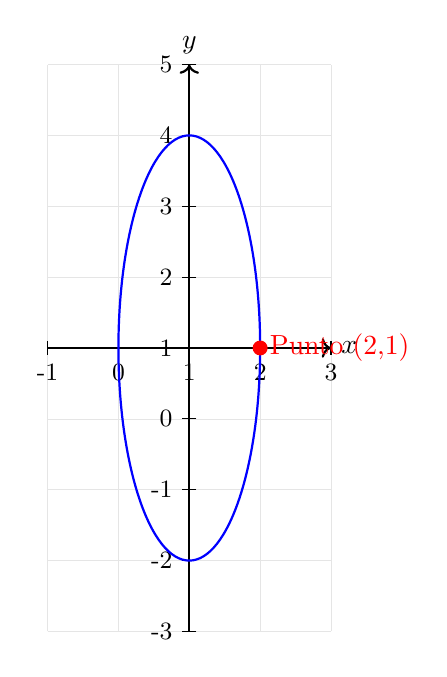
\begin{tikzpicture}[scale=0.9]
    \draw[help lines, color=gray!20] (-1,-3) grid (3,5);
    \draw[thick, ->] (-1,1) -- (3,1) node[right] {$x$};
    \draw[thick, ->] (1,-3) -- (1,5) node[above] {$y$};

    \foreach \x in {-1,0,1,2,3}
        \draw (\x,1.1) -- (\x,0.9) node[below] {\small \x};
    \foreach \y in {-3,-2,-1,0,1,2,3,4,5}
        \draw (1.1,\y) -- (0.9,\y) node[left] {\small \y};

    \draw[blue, thick] (1,1) ellipse [x radius=1, y radius=3];
    \fill[red] (2,1) circle (3pt) node[right] {Punto (2,1)};
\end{tikzpicture}
\caption{Radios vectores = 3 y 3}
\end{figure}
\newpage

\subsection{Ejercicio 17}
\textbf{Enunciado:} El punto medio de una cuerda de la elipse \(x^2 + 4y^2 -6x -8y -3 = 0\) es el punto \((5,2)\). Hallar la ecuación de la cuerda.

\textbf{Solución paso a paso:}
1. Reducción:
   \[
   (x-3)^2 + 4(y-1)^2 = 16 \implies \frac{(x-3)^2}{16} + \frac{(y-1)^2}{4} = 1
   \]
2. Fórmula de cuerda con punto medio \((x_1,y_1) = (5,2)\):
   \[
   \frac{(x-3)(5-3)}{16} + \frac{(y-1)(2-1)}{4} = \frac{(5-3)^2}{16} + \frac{(2-1)^2}{4}
   \]
   Simplifica:
   \[
   \frac{x-3}{8} + \frac{y-1}{4} = \frac{1}{2}
   \]
   \[
   x + 2y = 9
   \]

\textbf{Gráfica:}
\begin{figure}[H]
\centering
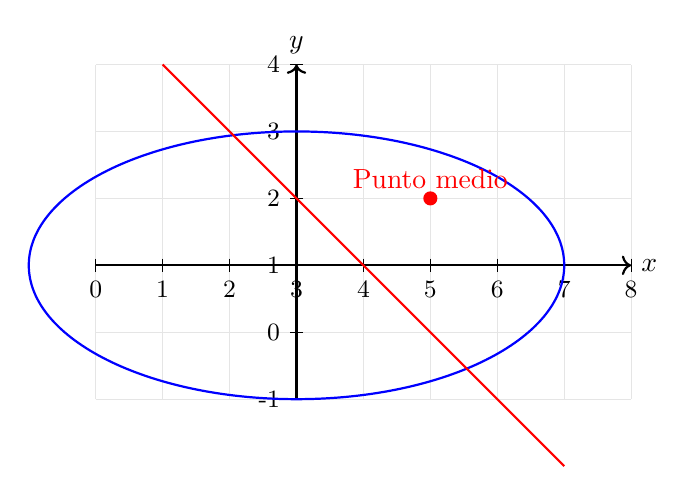
\begin{tikzpicture}[scale=0.85]
    \draw[help lines, color=gray!20] (0,-1) grid (8,4);
    \draw[thick, ->] (0,1) -- (8,1) node[right] {$x$};
    \draw[thick, ->] (3,-1) -- (3,4) node[above] {$y$};

    \foreach \x in {0,1,2,3,4,5,6,7,8}
        \draw (\x,1.1) -- (\x,0.9) node[below] {\small \x};
    \foreach \y in {-1,0,1,2,3,4}
        \draw (3.1,\y) -- (2.9,\y) node[left] {\small \y};

    \draw[blue, thick] (3,1) ellipse [x radius=4, y radius=2];
    \draw[red, thick] (1,4) -- (7,-2);
    \fill[red] (5,2) circle (3pt) node[above] {Punto medio};
\end{tikzpicture}
\caption{Cuerda \(x + 2y = 9\)}
\end{figure}

\newpage

\end{document}